    \chapter{Bourne shell}
    \section{簡介}
    shell是一個接受使用者命令後,請求作業系統執行的一個應用程式,有人會把shell
    畫畫包在kernel外面然後在包一層AP,我比較不贊同這種畫法啦,
    對於我來說shell也只是另外一種application程式而已,其實它跟gimp, netscape
    等等是一樣的東西,只是會被login叫出來。所以他是可以替換的一種應用程式。
    用C program來想,這樣子還可以幫你了解環境變數。
    \begin{center}
    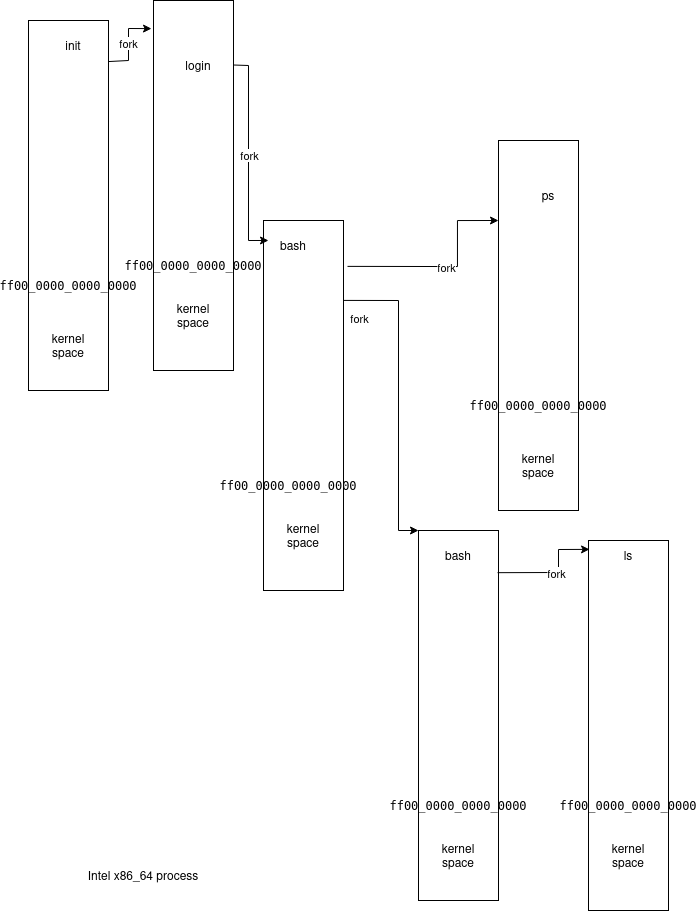
\includegraphics[width=10cm,height=13cm]{images/shell.png}
    \end{center}
    寫一隻shell其實非常簡單,主要是捉到user打的命令後,用fork跑出另一process
    (記住unix like是多人多工的然後在要這個child process用exec去執行這個
    外部程式例如ls, rm...等等。所以shell內部的運作大概是這樣的)
    \begin{enumerate}
    \item shell程式利用/dev/tty控制住鍵盤螢幕
    \item 打出prompt等待使用者輸入命令
    \item 捉到使用者輸入
    \item fork()一個新process
    \item exec()命令
    \item 執行完這個命令又回到shell
    \end{enumerate}
    在這邊您會看到unix like的執行一個程式都是藉由exec這個system call來執行的,
    這是作業系統提供使用者程式執行程式的機制。system call是user程式跟kernel
    溝通的管道。
    \\\\
    在以前MS DOS時代,一開機後會去執行command.com這隻程式就是shell。
    他就會跑出
    \begin{verbatim}
    C:\>
    \end{verbatim}
    等使用者輸入命令,這個C:就是提示符號(prompt),bourne shell通常prompt是\$,
    只不過這個dos shell功能相當的差,所以當時有個很有名的4DOS這個shell可以取代
    他。(4DOS這個shell其實拿了很多unix上shell的特性。當然跟真的unix shell還是
    不能比) 如果您只是用老鼠按一按一些icon,後來的MS-Windows時代,X的時代的
    command line shell就被圖形化的介面給取代了。不過執行另一個程式的機制還是一
    樣,還是要exec()。
    \\\\
    unix like 的系統的命令交談式的shell基本上除了能執行外部命令,主要他可以
    ''解釋''一些字串來執行,這些字串script的好處是可以設定一些環境。
    把多個外部命令集合起來完成一件工作。
    例如在Windows下我們也會設定TMPDIR這樣的目錄指到那個目錄去,有些windows程式
    會把執行中的一些暫時檔案放在這裡。unix like的shell scripts語法可以有if, 
    while, for loop等等,搭配一些外部命令,可以隨著環境不同時有不同的設定,
    使得一些日常工作維護更得心應手,比老舊的dos shell更為強大。
    \\\\
    sed, awk....,這些外部工具久而久之已經算是標準的unix系統必備的命
    令工具,就像winzip可能變成每個windows都會裝的工具。很多工具算是不成文的內定
    輔助shell programming工具了。所以真正說起來shell programming不單單是光
    懂shell的語法而已,而是要懂其他程式的選項,語法拉拉雜雜的一堆東西。
    \subsection{執行shell script與subshell}
    兩種方法
    \begin{itemize}
    \item 喚起新shell再執行shell scripts
    \item 在目前shell執行shell scripts
    \end{itemize}
    喚起另一個shell來執行的scripts在scripts檔頭最前面前要加
    \begin{verbatim}
      #! /bin/sh
      #! /bin/bash
    \end{verbatim}
    使用 sh 跟 bash 會有不一樣的行為,bash 會有比標準 sh 更多豐富的語法支援。
    \\\\
    第一種方法是在shell script 文字檔前指出shell scripts解讀的程式在那(也就是
    我們的shell)然後把文字檔的執行權限打開,照一般執行可執行檔方式執行或者叫
    一個shell來解釋文字檔test.sh。
    \begin{verbatim}
      $ test.sh
      $ /bin/sh test.sh
      $ ( . test.sh; )
      $ exec test.sh
      $ cmd1 | cmd2 | cmd3
    \end{verbatim}
    第二種方法是用命令''.''或者source執行。
    \begin{verbatim}
      $ . test.sh
      $ source test.sh
      $ { test.sh; }
      $ eval '. test.sh'
    \end{verbatim}
    差別在於一些設定只有在這個shell下的才算數,而喚起另一個shell就是另一個
    不相干的世界,
    也就是用第一種方法執行的script中變數的設定,不會影響到原來的shell變數。
    這個相當重要,其中很重要的是pipeline執行是喚起每個subshell來執行命令,
    然後把stnadard in standard out 串接,但是在各個subshell的變數是不互通的。
    ksh沒有source這個命令,所以最好不要用source。
    中括號( )表示用另一個subshell大括號,\{ \}表示用目前shell。例如
    \begin{verbatim}
      $ ( VAR='testvar'; )
      $ echo $VAR

      $ { VAR='testvar'; }
      $ echo $VAR
      testvar
    \end{verbatim}
    只有\{ \}內的VAR中的值被設定。其中用 . 的方法要很小心,
    不要在script裡面用
    \begin{verbatim}
      $ . test.sh arg1 arg2
    \end{verbatim}
    因為arg1 arg2會繼承呼叫這個script的arg1 arg2來,用 . 的方式最好是要執行
    的script只是一團script library不帶參數。
    另外如果 . test.sh執行,test.sh離開時,呼叫. test.sh的shell也跟著離開。

    \section{變數函數與模組化寫作}
    \subsection{變數使用}
    給變數值用
    \begin{verbatim}
      var="value"
      var='value'
      var=`command`
    \end{verbatim}
    要把值拿出來要加個錢符號\$
    \begin{verbatim}
      $ var="I am a gyoza"
      $ echo $var
      I am a gyoza
      $ var=`ls *`
      $ echo ${var}

      $ var='$var'
      $ echo $var
      $var
    \end{verbatim}
    以上要注意的是空格是有差別的還有引號的不同與作用。請往下看
    \subsection{引號quote}
    鍵盤上的double quote, single quote, backquote要弄清楚。
    \begin{itemize}
    \item backquote `command` 這個是命令取代,跟 \$(command)很像。
          所以常常看到var=`command或者var=\$(command),
          就是把command執行結果設給var。backquote會作反斜線的escape但
	  是\$(command)不會,所以如果有double scan變數時要小心。
    \item single quote 在' '內的文字通通保持原樣不做代換,有些保留符號在單引號
          內不再保留特殊意義。
    \item double quote 在" "內的文字\$ ` "三種意義會代換,其它的保持原樣
    \item escape char  在\verb=\=  後的單一字元也可以保持原樣
    \item 但是要escape ' ",就無法用反斜線,而是需要交互使用"跟',主要是shell
          的字串跟C一樣,是可以自動連結的,"string1"'string2' 就會變成
          string1string2,所以必須使用交互使用的"'"'"'來escape掉' 與 ",
          echo "'"'"'玩一玩。
    \end{itemize}
    \subsection{中括號的變數取代}
    加上括號\verb={}=是parameter的方法,
    \verb=${var}=是比較好的寫法,如果沒有要加其他字串可以用\$var就好。
    小心空格是有差的,他不像其他程式寫作,多空一個與少空一格是有差的。
    其他變數一些用法:
    \begin{itemize}
    \item \$\{var:-value\} 如果var有值了那麼就用原本的值,不然用value的值
    \item \$\{var:+value\} 如果var有值就用value的值
    \item \$\{var:?message\} var有值那麼就用原本的值,不然就印出message
      值到螢幕並且跳出。
    \item \$\{var:\%pattern\} 如果pattern與var後面的部份吻合,傳回剩下沒有
      吻合部份給var
    \item \$\{var:\#pattern\} 如果pattern與var前面的部份吻合,傳回剩下沒有
      吻合部份給var
    \item \$\{var/pattern/substitute\} 如果var有pattern吻合就代換成substitute
    \item \$\{\#var\} 這是字串長度,相當於strlen(var);
    \item \$\{var: offset:length\} 這是substring, \$\{var: -4:2\}
      表示從屁股第四個字元處拿回兩個字元。由於- 在前面是有用途的,所以要從屁股
      拿時,必須冒號後面空一格。
    \end{itemize}
    請看一個例子
    \begin{verbatim}
      # remote shell $RSH會等於/usr/bin/rsh  如果RSH當初沒有給值
      RSH=${RSH:-/usr/bin/rsh}

      # :+ 這種方式用在可有可無的option很好用
      # 以下面這個副程式為例子
      # 如果傳參數給他則VAR變成"-o 參數",沒有參數則VAR沒有值
      # $1 是第一個傳進來的參數  如果有值VAR就用"-o $1"
      func()
      {
          VAR=${1:+" -o $1"}
      }

      # :% 這種可以用在擷取字串的某部份
      # 例如  find 或者有的命令取回的結果往往是絕對路徑名
      # 但我們只想要最後面的那個檔案名時可以用這個來擷取
      # 不過傳統的bourne shell沒有% # pattern match,這只有在
      # ksh bash才有 最好不要用改用sed比較保險一點

      PRIV_HOST=fermion-priv
      PUB_HOST=${PRIV_HOST:%-priv}
      echo $PUB_HOST
      (PUB_HOST會等於fermion)

      # 代換也是  在新的Korn shell與Bourne Again Shell上才有
      
      BLOCK_DEVICE=/dev/vx/dsk/oracledg/vol_0
      RAW_DEVICE=${BLOCK_DEVICE/dsk/rdsk}
    \end{verbatim}

    \subsection{環境變數}
    普通的變數 如果Bourne shell, korn shell下用 \\\\
    \$ export var \\\\
    c shell, turbo c shell用 \\\\
    \$ setenv var \\\\
    則這個變數就變成一個環境變數。在C裡面的\\

    main(int argc, char **argv, char **envp)\\ 

    我們可以在shell裡設環境變數,而這個值是每個由這個shell fork出的程式,
    經由envp都看得到的。這個argv, envp指的都在virtual memory的下面stack
    往上長的開始處。
    所以shell也不過是一個"User space的C program",環境變數藏在C image user 
    space最下面,也可以從getenv這個library function call拿到。
    所以一般光設變數,沒有設環境變數沒有辦法把值告訴其它的程式。
    這邊要注意的是原本的Bourne shell的export沒有支援\\\\
    \$ export var=value\\\\
    的寫法,所以看到一些shell scripts為了portable起見都用\\\\
    \$ var=value \\
    \$ export var \\
    \subsection{一些內定變數}
    \begin{itemize}
    \item \$? 前一個命令執行完的status,
      0表示沒問題,在程式設計裡,0表示FALSE也表示No ERROR,所以程式的exit
      與return要處理好
    \item \$\# 表示傳給shell的arguments數量,這常跟\verb=set --=合用。
    \item \$0 這個shell命令名字
    \item \$1 \$2 \$3 ... function傳進來的參數arguments,
    \item \$@ 表示function 傳進來的所有arguments,如果加上double quote會等於
      "\$1" "\$2" "\$3"
    \item \$* 表示function 傳進來的所有arguments,如果加上double quote會等於
      "\$1 \$2 \$3"。 如果IFS有設值的話,例如 : ,那會是"\$1:\$2:\$3",所以使用
      for p in \$*; do echo \$p; done 跟 for p in "\$*"; do echo \$p; done
      的結果是不一樣的。
    \item \$\$ 表示目前的process ID
    \end{itemize}
    這邊\$@ \$*是不一樣的要小心double quote的不一樣,用*是會變成單一值的。
    \$?用在測試條件的判定是最常用的。
    \\\\
    shell一開始也會設定一些內定環境變數,這些環境變數會有一些程式自動會來讀取,
    例如mail程式用的MAIL,還有指明命令所在搜尋目錄的PATH等等。
    這些是寫bash, ksh, csh的C一開始寫在C程式內的。
    看環境變數用env這個命令,看變數用set命令就看得到不一樣結果。

    \section{函數與多檔模組化}
    函數的定義很直接就是
    \begin{verbatim}
func()
{
    cmd
    cmd
    ...
    return 0;
}
    \end{verbatim}
    傳值也是一樣的道理\$1 \$2 ...\$@ 等用法是一樣的。
    呼叫時就是
    \begin{verbatim}
func arg1 arg2 ...
    \end{verbatim}
    要注意的是變數是沒有像C一樣的有local variable,通通是global的。
    簡單的perl也是這樣。bash 有提供 local 修飾,但也不是傳統 sh 通用的。
    \\\\
    return 數字會變成\$?這個變數,return 字串沒有意義。在function內用echo
    會輸出到standard out。要作function執行後的判斷,可以用\$?或者讓他echo
    一些字串當成true。
    \subsection{模組化程式}
    function是最簡單的modulized寫作,再來就是多個模組檔當成shell lib檔。
    用了多個檔的問題跟C是一樣的就是變數怎樣在一個檔定義了,然後讓別的檔參照。
    通常export 成一個環境變數或者用eval這個內部命令執行一個個shell script使得
    這變數是大家都看得到的。

    \section{重要外部與內建命令}
    我們常用的ls, cp, sh....等等這些都是一個可執行檔,相對於一個外部可執行檔,
    shell有一些內建的命令藏在shell裡面,這些是built-in的內部命令是當初用C寫
    shell這隻程式時就寫在裡面的,像cd, export這就是。
    \\\\
    bash其實有很多以前的外部命令他都包含進來作成內部命令了,例如echo, getopts,
    不過為了程式可攜性,我們還是把他們稱為外部命令。這些內建命令可以用enable, 
    disable在bash內取消掉。不過別的sh, ksh或許就沒有了。要小心。
    \subsection{內建命令}
    比較重要且難一點的內建命令有
    \begin{itemize}
      \item : 假指令,甚麼都不作,等於CPU內的NOP指令。
      \item eval 大部分用來作兩次變數替換
      \item exec 執行某種命令並且替換掉目前shell(原本的執行不會替換掉shell)
      \item read 得到使用者從standard in(鍵盤)輸入
      \item set shell的精細設定,例如debug shell scripts
      \item test shell scripts的控制語法內的測試條件
      \item trap 接到某種訊號的處理
      \item shift arguments的處理
    \end{itemize}
    \subsubsection{ : magic numbers與註解}
    :是不做任何事的,在Unix中系統要執行程式會去檢查檔案前的字串叫
    magic number,古老的Bourne Shell的執行magic number是 : 而不是 \#!
    所以看到這種以:開頭的shell script可就要肅然起敬,同時:也有人拿來作註解用
    而不用\#的,主要是這可以拿來做大段落的comment,這特別要用單引號
    \begin{verbatim}
: << 'BLOCK_COMMENT'
blablabla
blablabla
alibuda
BLOCK_COMMENT
    \end{verbatim}
    這些老習慣的shell script可都是很厲害的。
    \subsubsection{eval與脫逃字元}
    eval可以拿來執行一個命令,不過他最常用的是拿來作兩次變數的代換,
    主要是每次執行一個shell
    命令他會先evaluate一次,看到有\$這個東西的就把值換一次把變數換掉,
    然後再執行一遍。這種double scan的方法對一些變數代換很有用,
    因為eval不是喚起另一個shell來執行,而是在本來這個shell內多evaluate一次,
    所以代換結果可以保留下來。
    例如如果我們要兩次代換
    \begin{verbatim}
      count=1
      var1=I
      var2=am
      var3=a
      var4=gyoza
      while [ $count -lt 5 ]; do 
         eval "echo \$var$count"
         let 'count=count + 1'
      done
    \end{verbatim}
    count可以一直變化1. 2. 3 ....要產生一個新變數var1 var2 var3....然後再對
    var1 var2取值。其中因為第一個var不想被運算,所以先用escape字元\verb=\=,
    然後第二次運算時才被解釋。
    那如果要三次以上變數代換在一行內解決呢? 想想看吧。要注意的是backguote跟
    \$(command)在double scan的不同,只有backquote會作反斜線\verb=\=的代換。
    \\\\
    eval主要還用來evaluate執行一個shell script檔,可以像C一樣寫成很多的
    模組shell script在同一個shell下run,則變數在此shell內通通有效。
    \begin{verbatim}
    $ eval ". foo.sh"
    \end{verbatim}
    不過如果變數太多,名字會打架。
    \subsubsection{exec}
    exec 會把''目前''的shell整個process拿掉,換成後面的命令,其實這就是用
    exec()這個system call置換掉子行程的意義是一樣的。
    最常看到是在~/.xinitrc這個scripts中置換掉成window manager。例如
    exec twm。
    所以如果你在shell中執行
    \begin{verbatim}
      exec cmd
    \end{verbatim}
    而cmd這個命令不存在就會回到login去,因為整個shell被換到cmd,但卻沒
    有cmd這個執行檔。
    所以執行程式的方法兩種是不一樣的
    \begin{verbatim}
      $ exec cmd
      $ cmd
    \end{verbatim}
    放在scripts的執行當然也不一樣。
    不過exec在script有另一個相當重要的用途就是跟file descriptor的連結,
    這個等下面再來討論。
    \subsubsection{read}
    \begin{verbatim}
    $ read input
    read from standard input
    $ echo $input
    read from standard input
    \end{verbatim}
    則會停在這邊等待鍵盤輸入,輸入字串變成\$input這個變數的值。
    \\\\
    其實read是等著從standard input拿東西進來,請記住是目前這個shell的standard
    input,所以像下面的作法是沒有辦法給變數值的
    \begin{verbatim}
    pipeline其實是叫sub shell執行每一道命令,此var是在另一個subshell中

    $ find . | read var

    用( )是喚起另一個subshell

    $ ( read var )
    \end{verbatim}
    \subsubsection{set}
    set通常是拿來設定這個shell的執行環境的。所以set跟環境變數中的值有很大關係,
    他後面的arguments會自動分到\$1 \$2 ....。比較重要的script會用到的大概
    \begin{itemize}
    \item set \verb=--= 正常看到-後面是option,現在不再是option
		而是一個命令參數。如-1 -2 ...這個可以變成一個參數。
    \item set -a 從這邊以後變數自動變成環境變數。
    \item set -f 不要解釋檔名的特殊字元例如wildcard *不再解釋為所有的意思了。
    \item set -x debug shell scripts
    \item set -o ignoreeof   一定要用exit離開shell,本來按Ctrl-D(eof)也可以
    \item set -o noclobber   關掉I/O導向不準overwrite檔案
    \item set -o notify      shell結束時報告background job的status
    \item set -o noglob      關掉wildcard字元解釋 如 * ? [ ]
    \item set +o 把-o的反向操作
    \item set -  關掉-v -x \verb=--=三種選項
    \end{itemize}
    set \verb=--= 或者set - 常常用在shell scripts裡面。其中set \verb=--=常用在
    set \verb=--= "val1 val2 val3",會變成\$1=val1 \$2=val2 \$3=val3。也就是
    \$*='val1 val2 val3'。如果後面沒有arguments,那就unset \$*。
    set -o 是很常用的例如set -o vi設定shell的操作方式用vi方法,
    取回上個命令就是按ESC再按k囉。 set -o emacs就是用 emacs 的方法 Ctrl-p 
    或上鍵。
    \subsubsection{test}
    test是控制語法中的測試條件,這個在下面討論。
    \subsubsection{trap}
    捉到某個signal時shell做的對應,
    \begin{verbatim}
    通式
    $ trap "command" signo
    其中signo是
    cyril@grill:~$ kill -l
 1) SIGHUP       2) SIGINT       3) SIGQUIT      4) SIGILL
 5) SIGTRAP      6) SIGABRT      7) SIGBUS       8) SIGFPE
 9) SIGKILL     10) SIGUSR1     11) SIGSEGV     12) SIGUSR2
13) SIGPIPE     14) SIGALRM     15) SIGTERM     17) SIGCHLD
18) SIGCONT     19) SIGSTOP     20) SIGTSTP     21) SIGTTIN
22) SIGTTOU     23) SIGURG      24) SIGXCPU     25) SIGXFSZ
26) SIGVTALRM   27) SIGPROF     28) SIGWINCH    29) SIGIO
30) SIGPWR      31) SIGSYS
    例如
    $ trap "" 2
    $ trap "rm $TMPFILE" EXIT 1 2 15
    \end{verbatim}
    如果""的command則表示shell不處理這個signal,
    2號就是INT通常就是按了Ctrl-C打斷shell script的執行,15就是
    TERM(process被kill了),再看難一點的例子
    \begin{verbatim}
trap_init()
{
        trap '  scriptcleanup
                [ "$SCRIPT_DISP" = ABORT ] && exit 100
                [ "$SCRIPT_DISP" = PASSED ]; exit $?' EXIT
        if [ -z "$__TC_INTERACTIVE" ]
        then
                for sig in HUP INT TERM; do
                        trap "  trap - HUP INT TERM;
                        echo 'Signaled - cleanup after script ...' >&2;
                        scriptcleanup $sig; kill -$sig $$; exit 101"  $sig
                done
        fi
        trap : PIPE
}
    \end{verbatim}
    這個例子的前面如果抓到EXIT這個signal就執行scriptclean到exit \$?的code,
    就是單quote內的東西,
    如果\$\_\_TC\_INTERACTIVE不是空字串,就執行下面的signal處理,
    如果是 trap - ,則表示回到最開始進入shell時的設定。
    最後如果是SIGPIPE(13號)就不做任何事(冒號:)
    那這有什麼好處呢,signal的處理相當於就是軟體中斷,在multiprocess時,
    可以可以成為兩個process間的彼此溝通。例如電動玩具的作法,通常一定有
    兩個process,一個負責鍵盤讀取,另一個負責一直重劃螢幕,所以就變成兩個
    process要互相溝通。有了trap,用shell都能寫文字電動玩具。

    \subsubsection{shift}
    shift是用來把進來的arguments移一個位移,
    shift n 移n個位移,
    shift可以拿來用超過10個以上的argrments,因為\$1 ... \$9只有9個而已。
    來看一個shell的queue list的append
    \begin{verbatim}
    # list_append list_name item ... - append items to a list
    list_append()
    {
        _list_a_name=$1; shift
        eval "set -- \${$_list_a_name} \$*"
        eval "$_list_a_name=\$*"
    }
    \end{verbatim}

    \subsection{外部命令}
    有些外部命令常用到
    \begin{itemize}
    \item basename 拿掉副檔名的處理
    \item echo 印出message的方法
    \item find 找檔案
    \item getopts 處理傳進來的arguments,跟C函式庫的getopt()很像
    \item xargs pipe時的命令執行與參數arguments的處理
    \end{itemize}
    另外sed awk會有專門介紹。
    \subsubsection{basename}
    捉出檔名副檔名工具。
    \begin{verbatim}
    $ basename foo.c .c
    \end{verbatim}
    則副檔名 .c 會被幹掉
    \begin{verbatim}
    $ basename /dira/dirb/dirc/foo.c
    \end{verbatim}
    則會剩下foo.c
    \begin{verbatim}
    $ dirname /dira/dirb/dirc/foo.c
    \end{verbatim}
    會抓出/dira/dirb/dirc
    \subsubsection{echo}
    echo是印出東西到螢幕的手段(也有print, printf可以用),
    這邊要講的是sh, ksh內的echo與bash的不一樣,所以設定有些不一樣。
    \begin{verbatim}
    echo -n  "messages"     不要換行(newline)
    echo -e  "messages\c"   解釋escape字元\c,等於-n用法
    echo -e  "\t messages"  tab在messages前
    \end{verbatim}
    傳統sh, ksh是沒有-n -e選項的,直接用echo就好。
    \begin{verbatim}
    echo "messages"     要換行(newline)
    echo "messages\c"   解釋escape字元\c 不要換行(newline)
    echo "\t messages"  tab在messages前
    \end{verbatim}
    使用-n -e可以用來處理binary的資料,最常用就是用hex,例如
    \begin{verbatim}
    echo -ne "\x1b[32malibuda\n"   印出綠色alibuda
    chs="\x80\x21\x20\x00\x0c\xfe\xff\xff"
    echo -ne $chs | dd if=stdin of=/dev/sdc seek=446 bs=1 count=8
    \end{verbatim}
    對/dev/sdc第1 partiton資料直接修改。
    \subsubsection{getopt}
    getopts其實是ksh, bash的內部命令,getopt才是真的外部命令。
    這很像C裡的getopt()。請看個例子
    \begin{verbatim}
    while getopts :vp:x:y:d:T:X:Y: c
    do
        case $c in
        v) 
                VERBOSE=yes
        ;;
        p)
                PLOT_TEMPLATE="$OPTARG"
        ;;
        x)
                X_AXIS="$OPTARG"
        ;;
        y)
                Y_AXIS="$OPTARG"
        ;;
        T)
                TITLE="$OPTARG"
        ;;
        X)
                X_LABEL="$OPTARG"
        ;;
        Y)
                Y_LABEL="$OPTARG"
        ;;
        ?)       
                echo "$PROGRAM_NAME Error: $0 : Unrecognized option" >&2; usage;
                exit 2;
        ;;
        esac
    done

    shift `expr $OPTIND - 1`

    if [ $# -ne 1 ]
    then
        echo "$PROGRAM_NAME: must specify a multi-column data file"
        usage
        exit 1
    else
        DATA_FILE=$1
    fi
    \end{verbatim}
    其中冒號:是說這個參數一定要有跟著的參數值,沒有冒號像v表示後面沒有帶著參
    數值, 例如最常看到-v是說程式執行時是verbose mode就是這樣。
    \$OPTARG就是跟在後面的 參數,getopts自動幫我處理好,並且一個一個的丟進
    \$OPTARG來。他也有\$OPTIND跟C library的用法很像。
 
    \subsubsection{find}
    尋找檔案用的程式命令,
    \begin{verbatim}
    find . -name "regex"
    find / -type d 找directory
                 f 找plain file
                 l 找symbolic link
                 p 找named pipe file
                 b 找block device
                 c 找char device
    find . -perm 755
    find / -user cyril
    gzip `find . \! -name '*.gz' -print`

    not ! 有的shell要加\ 因為!有特別意義,例如bash表示取回以前的命令。

    find -name -type -o -name
    \end{verbatim}
    在script中很多時候都是脫逃字元問題,常看到\verb=\=時都要想到這是脫逃字元。
    在script中 ()也有特別意義表示喚起另一個subshell來執行所以碰到()時也要用
    脫逃字元。或者合sed awk一起使用時也是一樣的道理。
    \subsubsection{xargs}
    xargs用來處理一些輸出結果要來當另一個輸入的arguments碰到的問題。
    例如
    \begin{verbatim}
      # find /usr/include/ -name "*.h" | xargs -n 2 diff
    \end{verbatim}
    -n2是指定有兩兩當成輸出變成diff的argumnets
    \begin{verbatim}
      # find /usr/include/ -name "*.h" | xargs grep '#ifdef'
    \end{verbatim}
    正常內定是輸出的一拖拉窟的結果,有用xargs時是一個一個餵給後面的命令
    \begin{verbatim}
      # find /usr/include/ -name "*.h" | xargs -i cp {} ~/include/
    \end{verbatim}
    -i 與 \{ \}可以把find的輸出的每一個當成cp的第一個argument,~/.就可以當成第
    二個argument。
    其實find裡面有-exec這個選項後面也可以用\{ \}表示一個一個餵給後面程式,而不是
    一拖拉庫的餵給後面程式。
    \begin{verbatim}
      # find /usr/include/ -name "*.h" -exec cp {} ~/include/
    \end{verbatim}

    \subsection{簡單數學}
    主要是拿來作counter的,有很多種方法,下面介紹三種,
    bash有個內建的let,
    例如
    \begin{verbatim}
let 'x = x + 1'
let 'x = x * 1'
    \end{verbatim}
    注意!!這邊等號右邊的x取值時不用加錢符號,而且在單quote內也可以有空格。
    ksh也有內建的,不過這不是每種shell都有的,
    比較保險的portable作法是用expr這個外部命令。
    請看例子
    \begin{verbatim}
 if [ "$KSH" ]
 then
        eval '
        add()
        {
                result=$((${1} + ${2}))
        }
        sub()
        {
                result=$(($1 - $2))
        }
        mul()
        {
                result=$(($1 * $2))
        }
        div()
        {
                result=$(($1 / $2))
        }
        inc()
        {
                eval "$1=\$((\${$1} + ${2:-1}))"
        }
        dec()
        {
                eval "$1=\$((\${$1} - ${2:-1}))"
        }
        '
else
        add()
        {
                result=`expr $1 + $2`
        }
        mul()
        {
                result=`expr $1 \* $2`
        }
        div()
        {
                result=`expr $1 / $2`
        }
        sub()
        {
                result=`expr $1 - $2`
        }
        inc()
        {
                eval "$1=\`expr \${$1} + ${2:-1}\`"
        }
        dec()
        {
                eval "$1=\`expr \${$1} - ${2:-1}\`"
        }
    \end{verbatim}
    這上面定義了一些副程式,可以在script裡面一樣像呼叫一般命令呼叫。
    \$((1+1))是一個subshell執行1+1並且傳回結果,下面例子讓我想起我的basic程式
    \begin{verbatim}
     i=0
     while [ $((i=$i+1)) -lt 10 ]; do echo $i; done
    \end{verbatim}
    不過\$(( ))這跟\$\{VAR\%value\}一樣只有ksh bash有, (( )) 在 bash
    中代表了數學 context ,裡面的 + - * / 還有 \verb=< >= == 都是像 c 一樣的
    數學運算。在if else 中也可以用。最好不要用在需要 portable 的shell程式上。
    副程式的position parameters \$1, \$2 ....跟平常script程式原則一樣。
    \\\\
    如果要更多的數學例如小數點的運算或者sin log等函數使用, 就用bc和awk吧。
    或者現在系統上一定都有 perl, python,也可以用
    \begin{verbatim}
    $ echo "$i $j" | awk '{print ($1 + $2) / 3.1415926}'
    $ echo "$i + $j / 3.1415926" | bc -l
    $ echo "" | awk '{print (i + j) / 3.1415926}' i=$i j=$j
    $ r=5; python -c "print('%.2f', (2 * 3.1415 * $r));"
    $ r=5; perl -e "print(2 * 3.1415 * $r);"
    \end{verbatim}
    ksh與bash都支援typeset,不過傳統的sh並不支援,bash還有declare這個內部命令,
    這兩個都是拿來定義這個變數是甚麼性質的很像C的宣告。不過為了portable能不用
    就不要用,還是用最基本的sh就好,如果真的要寫得很複雜就用perl, python吧,
    如果非常的嚴謹就用C囉。
    \begin{verbatim}
      $ typeset -i int_var
      $ declare -r constant
    \end{verbatim}
    int\_var被設成整數,如果給字串則int\_var的值會是0。如果用-r 
    則constant的值從現在起不能再被改了。

    \section{File descriptor與I/O導向}
    一個程式最基本的會自動開啟三個檔,操作時相對應的代號就是file descriptor,
    其實也就是跟作業系統開檔每次要到的file descriptor,是per process的
    \begin{itemize}
    \item 0  standard input   通常就是鍵盤
    \item 1  standard output  通常就是螢幕 buffer I/O
    \item 2  standard error   通常就是螢幕
    \end{itemize}
    stderr 跟 stdout 都是輸出到螢幕,差別就是 stdout 是 buffer I/O ,他會等到
    所有字元都準備好了,才輸出到螢幕, stderr 不是,是馬上就輸出到螢幕,因此
    在練習多工程式中,錯誤訊息都是要馬上丟出螢幕的。
    以前很常用的 pipe
    \begin{verbatim}
    p1 | p2 | p3 ...
    \end{verbatim}
    就是把每個 process 的 stdout 串成下一個的 stdin
    \\\\
    我們可以用I/O導向
    \begin{verbatim}
      $ cat file1 > file2
      $ pgr1 2> error
      $ dirs 2>&1 > /dev/null
      $ dirs > /dev/null 2>&1
    \end{verbatim}
    來將結果導向。導向跟pipe是不太一樣的,I/O導向是dup2()這個system call,
    而用pipe用的是pipe(2),所以導向的順序是重要的,如果是先導向/dev/null的表示
    先duplicate一個file descriptor跟/dev/null一樣,再
    執行dirs時所產生的standard error丟到standard out再到黑洞/dev/null去,
    就是甚麼也看不到。所以dirs \verb=2>&1 >= /dev/null跟 
    dirs \verb=> /dev/null 2>&1= 是不一樣的。
    \\\\
    既然是 process 的 fd,所以他其實最真實的規則是
    \begin{verbatim}
    (process 1) 1> (process 2)
    (process 1) 0< (process 2)
    \end{verbatim}
    只是 1 跟 0 省略不寫而已。 而後面接檔案的意思只是有個看不見的 process
    幫你開檔,產生的 stdin, stdout 。因此
    \begin{verbatim}
      $ cat file1 > file2
    \end{verbatim}
    是說 cat 這個程式把 file1 的內容印出到 stdout,然後把他丟給一個不知名的
    process 開了 file2 的 stdin 去,然後這個不知名的 process 把他的 stdin
    內容填入到 files 去。所以只是 bash 特別給的語法給使用者方便,這個語法通
    用有
    \begin{verbatim}
    p1 m>  file  p1 重新導向fd m 並且先把檔案虧空
    p1 m>> file  p1 把結果導向fd m並且append到檔案後
    p1 m<  file  p1 重新導向開file 的 process 的 stdout 到p1 fd m
    p1 m>&n      p1 把p1 process 的 fd m 丟給file descriptor n
    p1 m<&n      p1 從file descriptor n 拿東西給p1 process 的 fd m
    p1 m>&-      p1 close process fd m
    p1 m<<text   p1 把 fd m 導向,直到讀到下個text為止,請看 Here 文件章節。
    p1 m< <(p2)  p1 把 process 2 的 stdout 變成p1 的 fd m
    p1 m&>       bash 特有的語法 &> file 表示 > file 2>&1,這跟 >& 顛倒
    \end{verbatim}
    前面的 m 很多時候在 stdin, stdout 都是省略的,
    要注意的是有些後面只能接檔案,有的接file descriptor,還有
    接file descriptor時不能有空格。而
    \begin{verbatim}
    dirs > /dev/null 2>&1
    \end{verbatim}
    dirs 這個執行的 stdout 變成開 /dev/null 程式的 stdin,那後面的
    \verb=2>&1= 指的 是 dirs 呢?還是開 /dev/null 的 process 呢?
    以結果論來說是 dirs 這個 process 的 2 變成 dirs 的 1.
    \\\\
    exec 最常用在與file descriptor 的關聯這裡
    \begin{verbatim}
      $ exec 3> LOGFILE
    \end{verbatim}
    exec 在前面說到是執行某個程式,整個跳到那裡去,但在 shell 裡面就是自己
    這個 bash ,所以 exec 3 變成把自己 bash 的 fd 3,連到不知名程式開檔
    LOGFILE 的 stdin ,然後一樣道理而已。
    \begin{verbatim}
      $ exec 2>&-
      $ exec < infile
    \end{verbatim}
    因此其中各意義分別為把standard err關掉。 把目前shell的standard input變成
    infile,然後要導到fd 必須用 \verb=>&=。以下例子為把 fd 10 跟 newfile
    關聯起來
    \begin{verbatim}
      $ exec 10<> newfile
      $ ls /proc/$$/fd
      $ echo something >&10
      $ cat newfile
      $ read -r line <&10
      $ echo $line
      $ exec 10>&-
    \end{verbatim}
    注意file descriptor 1,2,3與導向符號的空格。空格的格式不是亂空的。還有
    fd 不等於 newfile,他是 system call 的 open/read/write 的 fd,一旦
    建立,只是當時狀態的 fd buffer,所以後來用別種方式加減 newfile,是
    無法影響 fd 10 的狀態的。
    \\\\
    而因此有的命令像 read 是從 bash 這個 process 的 stdin 讀東西進來
    \begin{verbatim}
    read -r line < myfile
    read -r line <&4
    \end{verbatim}
    很多工具程式都會提供從 stdin 輸入,從stdout 輸出的轉向功能語法,
    最常用的就是用 hypen - 表示 stdin,或者使用 Linux 中的 /dev/stdin
    /dev/stdout 表示目前 process 的 stdin stdout 的檔案。
    \begin{verbatim}
    cat - << file
    cat my.tar.gz | tar zxvf - myfile
    \end{verbatim}
    而
    \begin{verbatim}
    while read -r line; do echo $line done< <(process)
    \end{verbatim}
    這個重要意義就是後面 process 的 stdout 與前面 while do done 的 shell
    process stdin 的連結,用 () 執行程式在以前說過是在另外個 shell 呼叫這個
    程式。這很重要的是如果process 輸出是一行一行的,那 while read 也是一行
    一行讀進來,這在字串中避開含有空白做為分隔 dlimiter (IFS) 是很有用的技巧。
    如果是
    \begin{verbatim}
    while read -r line; do echo $line done 10< <(cat file | grep 'we want')
    \end{verbatim}
    就是讀進 while; done 的 fd 10,但當我們故意用
    \begin{verbatim}
    $ read -r line 100<& <(ls)
    bash: /dev/fd/62: ambiguous redirect
    \end{verbatim}
    出現 error ,表示 <(ls) 其實是被 expand 成 /dev/fd/62 這個神奇檔案。所以
    語法錯誤。這個 <(process) 語法主要是找最後一個有空的 fd 變得很重要,在 C
    程式中也是一樣,man dup 時可以看到他很強調這點,在 Linux 中,一個
    process 的有空的 fd 可以從
    \begin{verbatim}
    /proc/$$/fd
    /proc/self/fd
    \end{verbatim}
    下面看到,但只有 Linux 提供這個 /proc 檔,所以為了程式可攜性,在BSD, 
    SystemV AIX, Solaris ... 能跑,還有建立這種有 ID 的物件,都不要忘了多工
    搶資源的情況,一定要透過系統幫你做 atomic 運算,確保這個 ID 是獨一無二
    ,因此 bash 提供了
    \begin{verbatim}
    $ exec {var}>hellofile
    $ echo ${var}
    \end{verbatim}
    表示由 bash 幫你搶了一個關聯 hellofile 確保獨一無二的 fd 到 var 這個變
    數上。
    \\\\
    這個還有一個古怪的地方,正常講我們應該用
    \begin{verbatim}
    var=15
    exec ${var}>hellofile
    \end{verbatim}
    怎麼會少了錢符號?原來我們在使用變數來做 fd 也要小心,要用單引號把
    > 先框起來,做 eval var 那個變數擴展成數字先,才知道這是要做導向語法
    \begin{verbatim}
    eval exec ${var}'>'hellofile
    \end{verbatim}
    由於單引號的奇怪語法很彆扭,所以 bash 給了一個這語法同時解決上面三個問題
    。這個語法 ksh 早在 2006 就有, bash 要到 4.1 版以後才有,目前是
    KornShell 93r+, Bash 4.1α+, Zsh 4.3.4+ 以上才有。
    但這語法不是 POSIX 標準的,以新 2017 POSIX 標準來看,這還是不 portable
    的。

    \subsection{Here 文件}
    導向符號有個 Here 文件型的導向,
    \begin{verbatim}
    (process1)m<<XXX > file1
    alibuda
    2nd line
    asaburu
XXX
    \end{verbatim}
    表示兩個XXX中間夾住的文字都變成 process 1 的 stdin (m是0可不寫),然後導
    向 file1, 這有兩個好處,一個就是大片的多行文字定義可以用這方便處理,二
    就是大片文字等於是多行註解。
    \begin{verbatim}
:<<COMMENT
This is comment
comment multiple lines
COMMENT
    \end{verbatim}
    記得 : 是不做事,這樣就不用一個一個放 \# 在每行前面。
    \\\\
    自動ftp的 scripts 的例子,
    \begin{verbatim}
#!/bin/ksh
# A script to automate FTP transfer

HOST=ftp
USER=user
PASSWORD=password
FILENAME_PATTERN=remote_files
REMOTE_DIR=/usr/doc
LOCAL_DIR=/usr/local
# -i = non-interactive, -n = disable auto-login

ftp -i -n <<HERE
     open $HOST
     user $USER $PASSWORD
     cd $REMOTE_DIR
     lcd $LOCAL_DIR
     mget $FILENAME_PATTERN
     close
     bye
HERE
    \end{verbatim}
    注意\verb=<<=的用法,ftp的input會一直讀到HERE為止,open, user, cd, mget
    都是ftp中的命令。不過也可以把
    這些ftp命令寫成一個檔案然後ftp \verb=<= 檔案也行。
    \subsection{embedded其他script與資料檔}
    在上面的ftp的例子,我們可以看到 ftp 的命令可以嵌在shell script 裡面,
    同樣的perl script或者其他可以從 stdin 獲取資料的命令也可以嵌在 shell
    script裡面,只要善用\verb=<<=就好。
    請看例子:
    \begin{verbatim}
    while read column1 column2 column3
    do
            echo $column1 $column2 $column3
    done <<__ENDDATA__
    99      98 3.5
    300     298 4.9
    498     493 5.9
    699     698 7.6
    900     748 9.0
    1200    703 9.6
    1500    651 10.4
    1698    627 10.8
    __ENDDATA__
    \end{verbatim}
    while do done;裡面的read要從standard in讀,我們把他從standard in導到讀到
    \verb=__ENDDATA__=所以下面的資料就分別讀進column1 column2 column3。
    再看一個perl的內堪例子
    \begin{verbatim}
#! /bin/sh

    perl -x - $* <<'End-of-Perl-Script'
#!perl
        #
        # given absolute or relative pathnames, create symlinks from the
        # destination directory back to the source file(s) using relative
        # pathnames
        #
         
        if (@ARGV < 2) {
                print STDERR "must specify at least two files\n";
                exit 3;                                          
        }
        @srcfiles = @ARGV[0 .. @ARGV - 2];
        $targ = $ARGV[@ARGV - 1];

        if ($targ !~ m,/,) {
                $targ = "./$targ";
End-of-Perl-Script
    \end{verbatim}
    從這邊可以把perl用-x叫出來解釋perl的語法。

    \subsection{導向的用途}
    多工的 process 間資訊傳遞都是高級程式的重點,剛剛用的 file descriptor,
    其實就是多工 multiplexing 的最基本方法之一。可以從 parent process
    fork 出去的 child 連回 parent 來,兩邊互相送東西達成通訊功能。
    這在寫 shell 多工甚至一般 C 語言的多工都是一樣的道理。所以用 shell 是
    能寫電動玩具的,只要能一邊畫畫面,一邊接收按鍵,一邊處理運算這三個多工
    process 能溝通,就是一個標準的電玩程式。
    \\\\
    這種 file I/O 的多工,最基本的就是 pipe,某個 process stdout 變成另外
    process 的 stdin,這也可以用 mkfifo 建立一個有 in 跟 out 的特殊 fifo
    檔案,這也稱為 named pipe
    \begin{verbatim}
$ mkfifo inout
$ echo 'fifo in' > inout &
[1] 1763084
$ cat inout
fifo inout
    \end{verbatim}
    如果 inout 這個檔案裡面是空的,則一個 cat (read) 會 block 等在那裡直到
    inout 這個檔有內容進來。
    \\\\
    在一般使用上,可能最重要的多工是 terminal 的畫圖,例如 wget, curl
    下載檔案的 progress bar,這種一邊做某件事,一邊處理畫面都是多工應用
    ,即使是系統軟體在做長時間解檔,網路作業等跟 device 等待有關的程式
    也都會用到,這其實用 shell 就輕易的做到了。

    \section{流程控制與測試條件}
    \subsection{測試條件}
    在Bourne shell的內部命令裡面有測試條件的語法test給if while用
    \begin{verbatim}
    test condition
    或者 
    [ condition ]
    \end{verbatim}
    這個 condition 是process 程式丟出來的 status \$?,如果是 0 ,就是
    true,如果是非 0 就是 false。 為了與autoconf不要混淆,programmer
    比較喜歡用 test 不用中括號condition的方法。括號的用法請注意要有空格。
    例如
    \begin{verbatim}
    檔案測試條件
    test -f /etc/file      檔案是個一般檔案不是其他特殊檔案嗎
    [ -e file ]            檔案存在嗎
    [ -d /etc/ ]           目錄存在嗎
    [ -s file ]            檔案大小大於0嗎
    [ -r file ]            檔案可讀嗎

    字串測試條件
    [ "$string" ]          string有東西就返回true
    [ -n "$string" ]       string有東西(non-zero)返回true
    [ -z "$string" ]       string沒東西(zero)返回true
    [ "$s1"  = "$s2" ]     s1 等於 s2時返回true
    [ "$s1" != "$s2" ]     s1 不等於 s2時返回true

    數值條件  小心有多個-喔
    [ $num1 -eq $num2 ]    num1相等    num2 為true   
    [ $num1 -ne $num2 ]        不等    num2 為true
    [ $num1 -lt $num2 ]        小於    num2 為true
    [ $num1 -ge $num2 ]        大於等於num2 為true
    \end{verbatim}
    \begin{verbatim}
    多重條件
    [ ! -f "testfile" -o ! -r "testfile" ]
    [ test condition -o test condition ]
    !               表示not
    -a		    表示and
    -o		    表示or
    \end{verbatim}
    通常比較常用的又有portable的就是上面一些用法。bash 又給了特別的數學
    ((  )) 與字串 \verb=[[  ]]= 測試方法,在(( )) 中可以用 + - * /
    \verb/< > == && ||/ 等 c 語言的判斷符號,而且變數也不用\verb=$=符號,
    \verb=[[ ]]= 除了也可以用 == , != 外,還可以用 regex \verb/=~/,
    而且作用也不分別字串或數字,算是很方便。
    或者能用 if \verb=[[ ]]= -o \verb=[[ ]]= 這種寫法。
    但也是如果程式要能在標準的 sh 上跑,也是能不用就不用,否則還蠻好用的。
    美觀上來說用中括號condition比較好看,很多人為了 autoconf 的語法 portable 
    起見, 盡量用 test 的寫法。測試的結果當然放在\verb=$?=中,0 表示成功,
    其他值表示失敗。
    \\\\
    在shell script中也有可能看到有人用
    \begin{verbatim}
    if [ "x$VAR" = "xvalue" ]; then .....
    \end{verbatim}
    來作\$VAR是否是空的測試,尤其你如果先測試是否為空字串,
    再測試是那個值要做什麼,這樣就會作兩次測試划不來,用這樣作比較經濟。
    \\\\
    另外這跟perl字串與數值測試容易混淆,他跟perl剛好相反,而且perl沒有多-
    \begin{verbatim}
    perl語法
    if ($str1 eq $str2)
    if ($num1 == $num2)
    \end{verbatim}
    最後有個大比較,會一起列出shell perl c的差異來。(人老了記不住,我是這樣記
    ,以perl為基準eq是字,所以前後是string,==是符號所以前後是number,
    bourne shell是怪胎,剛好顛倒,eq還要加個-符號。==要少一個=)
    \begin{verbatim}
    C語法
    if (!strcmp(string1, string2))
    if (num1 == num2)
    \end{verbatim}

    \subsection{if 條件判斷}
    if test;then cmd1; elif test; cmd2; else cmd3 fi
    \begin{verbatim}
      if test
      then
        cmd1
        ...
      elif test
        cmd2
        ...
      else
        cmd3
        ...
      fi
    \end{verbatim}
    同樣注意寫成一行時的分號位置。尤其在寫Makefile時會用到。
    另外他的else if 是 elif, 跟 C 的 else if 不一樣。
    \\\\
    另外有種簡單的if用法
    \begin{verbatim}
    [ "$VERBOSE" ] && echo 'everything'  && 表示傳回true時執行&&後面動作
    [ "$VERBOSE" ] || echo 'nothing'     || 表示傳回false時執行||後面動作
    \end{verbatim}
    其實這就是
    \begin{verbatim}
    process 1 && proess 2
    process 1 || proess 2
    \end{verbatim}
    如果多個串接
    \begin{verbatim}
    process && process 2 || process 3
    例如
    echo 1 | grep 2 >/dev/null && echo haha || echo ahah
    \end{verbatim}
    則有 if else 的作用
    \\\\
    這邊有點要注意
    \begin{verbatim}
    [ "$var" ]
    如果是空字串傳回false 這其實很像
    [ -n "$var" ]
    -z 是如果是空字串傳回 true
    [ -z "$var" ] 
    \end{verbatim}
    這用在兩個以上 condition 連接有 not 的情況,不然光用 
    \begin{verbatim}
    [ ! "$v1" -o "$2" ]
    \end{verbatim}
    會分不清是先 not 還是 not 作用在整個有 -o 的情況。
    \\\\
    condition 由於是根據程式執行結果,但有的時候例如 find 這個程式,
    找不到檔案並不意味著執行失敗,只是找不到而已,所以找不到回傳的 \$?
    還是 0,這並無法幫我們做判斷,但有的命令成功了會在standard out 印出
    一堆字串,我們可以利用這樣的行為來作判斷,例如
    \begin{verbatim}
    if find . -name alibuda; then
        echo "I find it"
    fi
    \end{verbatim}
    是不行的,而要用
    \begin{verbatim}
      [ "$(find . -name gyoza.txt)" ] && echo "I Find It !!!"
    \end{verbatim}
    用\$(cmd) 很像用`cmd`,差別就是會不會做反斜線的替代escape,如果找到了,
    會印出這個檔案來所以雙引號裡面" "有值,中括號\[ \]就還回true囉。如果沒有
    雙引號,如果只有一個字串則會當成字串永遠為true,所以
    \begin{verbatim}
    $ [ 1 ]
    $ echo $?
    0
    $ [ 0 ]
    $ echo $?
    0
    \end{verbatim}
    如果有兩個以上,則shell把find丟出來的字串又當成命令,想去執行他,就發生
    錯誤了。
    \subsection{for loop}
    for var in \$list; do cmd1; cmd2; done
    \begin{verbatim}
      for var in $somelist
      do
        cmd1
        cmd2
      done
    \end{verbatim}
    注意寫成一行時的分號位置。尤其在寫Makefile時會用到。
    list是shell裡常用的一種方法,就只是很多小單位用空格或tab分開的資料就是。
    例如
    \begin{verbatim}
      ME="I am a gyoza"
    \end{verbatim}
    ME就是一個list(bash的man page用list表示一堆commnands,
    把word表示這裡的list,有的書或者ksh, sh的man page又不一樣。
    所以我很不喜歡去定義這些名詞,有時候爭論這些沒有意義
    捉到key point比較重要)for 敘述可以一次把一個元素餵給前面的var
    \begin{verbatim}
      for ELEMENT in $ME; do
        echo $ELEMENT
      done
    \end{verbatim}
    就會出現
    \begin{verbatim}
      I
      am
      a
      gyoza
    \end{verbatim}
    注意錢符號與設定變數使用變數的差異。
    \\\\
    bash 特別有像 C 的 for loop,所以要用(( )) 的方法。
    \\\\
    for (( i = 0 ; i < 10; i++)) ; do cmd1; cmd2; done
    \subsection{while loop}
    while test ; do cmd1; cmd2; done
    \begin{verbatim}
      while test;
      do
        cmd1
        cmd2
      done
    \end{verbatim}
    同樣注意寫成一行時的分號位置。尤其在寫Makefile時會用到。

    \subsection{case switch}
    \verb=case $var in *)cmd1; cmd2 ;; xx?)cmd3; cmd4 ;; esac=
    \begin{verbatim}
      case $string in 
           *) cmd1; cmd2
           ;;
           xx?)
              cmd3
              cmd4
           ;;
      esac
      case $answer in
           [Yy])
              echo 'yes'
           ;;
           [Nn])
              echo 'no'
           ;;
      esac
    \end{verbatim}
    case switch的用法,不像C的是整數的case switch而是可以有字串的喔,
    其中符合的字串條件用globbing的方式,也就是wildcard *, ?, \verb=[ ]=
    ,有的書上寫regular express是錯誤的。注意用一行寫出的方法。

    \section{bash 特殊資料型態}
    除了 (( )) 與 \verb=[[ ]]=的特殊用法外,
    一般程式語言很常用的 array 與 hash,原本 shell 是沒有的,就只是基本的
    字串用空白鍵分開的 list 而已。bash 提供 index array,他的literal
    \begin{verbatim}
    declare -a a

    a[0]='first'
    a[1]=2
    a=('first' 2)
    echo ${a[0]}

    for v in "${a[@]}"; do echo $v; done
    first
    2
    for v in "${a[*]}"; do echo $v; done
    first 2
    unset a
    \end{verbatim}
    帶有key 的 hash array
    \begin{verbatim}
    declare -A h

    h['key0']='value0'
    h['key1']=2
    echo ${h['key0']}

    for v in "${h[@]}"; do echo $v; done
    value0
    2
    for v in "${h[*]}"; do echo $v; done
    value0 2
    unset h
    \end{verbatim}
    使用@與*跟之前的 shell 變數一樣,用double quote時會有不同,*會變只有單一
    值,@會變成很多值。所以要用二維陣列,必須用*
    \begin{verbatim}
    twod=("${a[*]}" "${h[*]}")
    echo ${twod[0]}
    echo ${twod[1]}
    \end{verbatim}
    同樣如果是要在 portable 的機器aix, solaris, ...上跑的話,儘量用最原始的
    sh,這種array, hash 就最好不用。

    \section{結語}
    一般標準用shell是Bourne Shell後來延伸出Korn Shell,很多老一輩的工程師
    還比較喜歡用korn shell寫scripts。第一次碰到令人讚嘆的 sh script 就是
    老工程師用 ksh 寫的 testing script, 另外還有BSD的C shell,
    c shell 也造成一股風潮,尤其在很多system admin,這是因為在 1990 年代中
    Sun 的機器實在是賣的很好,在美國公司內的 admin 很會寫 csh 的 script,
    即使在台灣我做過 IC chip 的testing, testing 機器與教我的人也是 csh,
    所以大概以現在2017年,在 50 ~ 60 歲左右的人,很大部份用 c shell。
    我在幾家大公司中的 default shell 都是 csh, 後來 tcsh 加進很多不錯的特點。
    一直到現在,我們新進人員 default shell 還是 csh, tcsh,相關工具也一定有
    c shell 的 script,只是後來 Linux 大行其道,bash 慢慢聲勢浩大。以前剛進
    公司,配的是 Solaris 機器,後來只剩 Linux 機器,最後只給 laptop,遠端用
    Linux VM,自己去要一個 Linux VM 來用。
    Bourne Again Shell 把大家有的沒的特點拉拉紮紮放在一起。拜GNU/Linux之賜
    年輕一代的工程師很多喜歡 bash,不過要注意 portable 的 shell scripts 寫作。
    (只是我看其他unix like系統大概也都死的死逃的逃,bash也算蠻通用的了)
    sh, ksh bash是同一家族的,這幾個語法比較接近,不像tcsh csh是另一家族,
    差很多。
